%% Work in progress -- targeting ICRA.
%% Build:  latexmk -pdf icra_seek.tex     (or ./build.sh)
\documentclass[conference]{IEEEtran}
\IEEEoverridecommandlockouts

\usepackage{cite}
\usepackage{amsmath,amssymb}
\usepackage{graphicx}
\usepackage{booktabs}
\usepackage{tikz}
\usetikzlibrary{arrows.meta,positioning}
\usepackage{xcolor}
\usepackage[hidelinks]{hyperref}

\def\BibTeX{{\rm B\kern-.05em{\sc i\kern-.025em b}\kern-.08em
    T\kern-.1667em\lower.7ex\hbox{E}\kern-.125emX}}

\begin{document}

\title{Decoupling Bearing and Range for Language-Directed Object Approach\\
on a Low-Cost Mobile Robot: A Deployment Study\\
\large\normalfont{[Work in Progress]}}

\author{\IEEEauthorblockN{Tim Amado}
\IEEEauthorblockA{\textit{AI361 Robotics Project}\\
Manuscript in preparation --- affiliation and contact to be completed}
}

\maketitle

\begin{abstract}
We describe a language-directed object-approach behaviour deployed on a
TurtleBot3 Burger: a spoken or typed instruction such as ``go to the bottle''
causes the robot to rotate until it finds the named object, turn to face it,
drive toward it, and stop at a fixed standoff distance. The system pairs a
small local language model, used strictly as an intent parser, with an
open-vocabulary object detector for bearing and a planar LiDAR for range. Our
central design choice is to \emph{decouple} these two measurements: the robot
first centres the target visually, then reads range along its own forward axis.
This removes any dependence on camera intrinsics or camera--LiDAR extrinsic
calibration, at the cost of forbidding simultaneous steering and ranging.
The contribution of this work-in-progress report is less the architecture than
the deployment record: on this platform, every failure that mattered arose from
\emph{sensor timing}, not perception accuracy. We quantify a $2.1$\,s
end-to-end camera latency caused by publishing faster than the wireless link
could carry, and describe four control-loop defects --- including a range
filter that could latch permanently after a single spurious reading --- none of
which would have appeared in simulation. Preliminary trials stop within
$1.5$\,cm of a $0.35$\,m goal, but the evaluation is small and single-site, and
we state its limits explicitly.
\end{abstract}

\begin{IEEEkeywords}
mobile robots, open-vocabulary perception, sensor fusion, language grounding,
field deployment
\end{IEEEkeywords}

\section{Introduction}

Instructing a robot in natural language is attractive precisely because the
instruction need not specify the world. ``Go to the bottle'' names a goal whose
direction and distance are unknown until the robot looks. Executing it requires
three capabilities that are usually studied separately: interpreting the
utterance, locating the referent, and closing a control loop on it.

Recent work has made the first two dramatically easier. Instruction-following
systems built on large language models can decompose commands into executable
steps~\cite{saycan,codeaspolicies}, and open-vocabulary
detectors~\cite{yoloworld,owlvit,groundingdino} localise objects named by
arbitrary text rather than by a fixed label set. It is tempting to conclude
that the remaining work is integration.

Our experience says otherwise. We built such a system on a low-cost platform
--- a TurtleBot3 Burger with a monocular camera and a 360$^\circ$ planar LiDAR,
commanded from a laptop over Wi-Fi --- and found that the components behaved
close to their published characterisations while the \emph{integrated} system
failed repeatedly. Every failure that consumed real debugging effort was a
question of \emph{when a sensor reading may be trusted}, not of whether a
detector was accurate. The dominant one was latency: the camera feed ran
$2.1$\,s behind reality, so a search behaviour that stopped and looked was
reliably inspecting a view from two steps earlier. The symptom --- ``the robot
rotates past an object that is plainly visible on screen'' --- reads as a
detection failure and is not one.

This paper reports that experience. We describe the architecture
(Sec.~\ref{sec:system}), the decoupling of bearing from range that lets it work
without calibration (Sec.~\ref{sec:decouple}), the deployment findings
(Sec.~\ref{sec:findings}), and preliminary results together with an explicit
account of what they do not yet show (Sec.~\ref{sec:results}).

\section{Related Work}

\textbf{Language-conditioned robot behaviour.} SayCan grounds an LLM's
proposals in a value function over robot skills~\cite{saycan}; Code as Policies
has the model emit executable policy code~\cite{codeaspolicies}. Both treat the
language model as a planner. We deliberately take a narrower position: the
model performs a single extraction --- the target noun --- and no value it
produces reaches an actuator without being clamped or refused by ordinary code.
On a platform whose motion is bounded by a $0.4$\,s watchdog, we found this
restriction easier to reason about than to relax.

\textbf{Open-vocabulary detection.} CLIP-style image--text
alignment~\cite{clip} underpins detectors that accept free-form class names at
inference time~\cite{owlvit,groundingdino,yoloworld}. We use
YOLO-World~\cite{yoloworld} for its real-time inference, which matters here
because the detector sits inside a control loop rather than an offline pipeline.

\textbf{Vision-language models for control.} We considered and rejected a VLM
in the loop. The requirement is a bounding-box centroid at close to camera rate;
a model that returns prose after seconds per frame cannot serve a robot that is
moving while it waits. This is a statement about our latency budget, not about
VLM capability.

\section{System Overview}
\label{sec:system}

\begin{figure}[t]
\centering
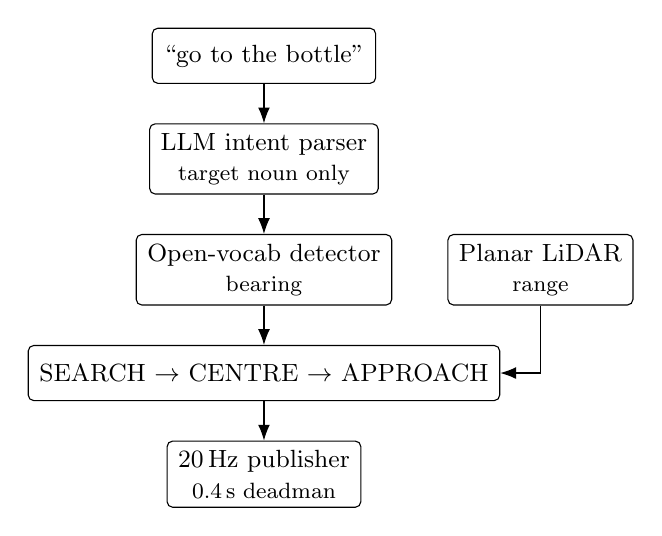
\begin{tikzpicture}[
  font=\small,
  box/.style={draw, rounded corners=2pt, align=center, minimum height=7mm,
              inner xsep=4pt},
  ar/.style={-{Latex[length=2mm]}}
]
\node[box] (utt) {``go to the bottle''};
\node[box, below=5mm of utt] (llm) {LLM intent parser\\{\footnotesize target noun only}};
\node[box, below=5mm of llm] (det) {Open-vocab detector\\{\footnotesize bearing}};
\node[box, right=7mm of det] (lid) {Planar LiDAR\\{\footnotesize range}};
\node[box, below=5mm of det] (fsm) {SEARCH $\rightarrow$ CENTRE $\rightarrow$ APPROACH};
\node[box, below=5mm of fsm] (dead) {$20$\,Hz publisher\\{\footnotesize $0.4$\,s deadman}};

\draw[ar] (utt) -- (llm);
\draw[ar] (llm) -- (det);
\draw[ar] (det) -- (fsm);
\draw[ar] (lid) |- (fsm);
\draw[ar] (fsm) -- (dead);
\end{tikzpicture}
\caption{Pipeline. The language model contributes only the target noun; it
never observes an image and never produces a velocity. Bearing and range come
from different sensors and are consumed at different times
(Sec.~\ref{sec:decouple}).}
\label{fig:pipeline}
\end{figure}

The platform is a TurtleBot3 Burger running ROS~2 Humble. A laptop subscribes to
a compressed camera stream, wheel odometry and a 360-beam planar LiDAR
(range $0.12$--$3.5$\,m), and publishes velocity commands over Wi-Fi.

A typed instruction is routed deterministically: a regular expression decides
whether it is a drive command or an approach command, and only then is a
language model consulted. This matters more than it appears. Both parsers use
constrained decoding against a JSON schema, and under constrained decoding every
schema property is effectively required; adding a \texttt{target} field to the
shared driving schema caused a 3B model to invent a target for commands such as
``forward 1\,m''. Two schemas with deterministic routing avoids the failure
entirely and leaves the existing driving prompt unmodified.

Motion is executed by a single-threaded arbiter that permits one bounded,
cancellable motion at a time. The approach behaviour runs \emph{on} that
arbiter's thread rather than beside it, so that a stop request, a manual
teleoperation command, and the $0.4$\,s command watchdog retain their existing
semantics without being aware that an approach behaviour exists.

\section{Decoupling Bearing from Range}
\label{sec:decouple}

A monocular camera cannot measure distance to an object of unknown size, and a
planar LiDAR cannot identify one. The conventional remedy is to calibrate the
camera and project detections into the LiDAR frame, which requires intrinsics
and camera--LiDAR extrinsics.

We avoid this. The behaviour first rotates until the detection's horizontal
centroid lies on the image centre line, then reads range along the robot's
forward axis. Once the target is centred, ``how far is the target'' and ``what
is in front of me'' are the same question, and the answer requires no knowledge
of the camera's field of view. The camera on our unit is mounted rotated and its
publisher applies a $90^\circ$ correction; the effective horizontal field of
view is therefore the sensor's narrow axis. Under a projection-based scheme this
would have to be characterised. Under ours it affects only the search step size.

The price is a constraint that took us some time to accept: \textbf{the robot
must not steer and range simultaneously}. While turning, the forward sector
sweeps across the scene and every reading describes something that merely
happens to be passing through it. An early version evaluated its stop condition
during such a turn and reported arrival at $0.26$\,m while standing $0.69$\,m
from the target. The behaviour now aims in place, and only reads range once
aimed.

\subsection{Range estimation}

Range is the $20$th percentile of valid beams in a $\pm10^\circ$ forward sector
--- a robust minimum, deliberately not a median. Measured on our unit, that
sector returned a minimum of $1.97$\,m against a median of $2.60$\,m: the median
described the wall \emph{behind} the object while something sat two-thirds of a
metre nearer. For a stopping criterion the nearest object in the path is the
only correct quantity. A percentile rather than a bare minimum is used because
isolated spurious short returns are common; in a representative scan only $251$
of $360$ beams were valid, with a dropout at the beam pointing directly ahead.

Thin targets can vanish from a tight sector entirely --- a chair at $2.6$\,m
produced zero valid beams within $\pm5^\circ$ --- so the sector widens to
$\pm20^\circ$ when the narrow one is unusable. Widening is safe in the direction
that matters: since the estimate is a minimum, a wider sector can only report
something nearer, and erring near means stopping early.

\section{Deployment Findings}
\label{sec:findings}

\subsection{Latency dominates, and is self-inflicted}

The most consequential defect was not in our code. The camera node published at
$30$\,FPS over a wireless link that carried approximately $7$; the surplus
queued, and the backlog \emph{was} the delay. We measured end-to-end latency by
issuing a rotation command and timestamping the first video frame whose content
changed:

\begin{center}
\begin{tabular}{lcc}
\toprule
Publish rate & First motion visible & Motion visible after stop \\
\midrule
$30$\,FPS & $+2.10$\,s & $+2.08$\,s \\
$5$\,FPS  & $+0.38$\,s & $+0.47$\,s \\
\bottomrule
\end{tabular}
\end{center}

The near-equality of the two columns at $30$\,FPS identifies a fixed transport
delay rather than jitter. Reducing the publish rate below the link's capacity
removed it: same camera, same network, one parameter.

Two consequences follow, and both were initially misdiagnosed as perception
failures. First, a step-and-look search that settles for less than the latency
inspects the view from a previous step; the robot rotates past a target that a
human observer can see on the video stream. Second, visual centring is a closed
loop on that delayed feed, so the robot continues turning blind for the duration
of the latency after the target reaches centre. Uncapped, at the platform's
$2.84$\,rad/s this is a blind arc exceeding $60^\circ$ through a frame roughly
$44^\circ$ wide: the target leaves the image and the loop reports it lost while
pointing directly at it. Capping angular velocity at $0.35$\,rad/s bounds the
blind arc below $8^\circ$.

We note the general form of this lesson: on a bandwidth-limited link,
\emph{publishing faster degrades control}, and the resulting failures present as
perception errors.

\subsection{A filter that could never recover}

To prevent the robot driving quickly at a target that is actually close, we
discarded range readings that jumped outward between consecutive samples.
Readings that jumped \emph{inward} were accepted unconditionally, since an
object entering the path must still be able to stop the robot.

This filter could latch permanently. Rejecting a reading left the reference
value unchanged, so a single spurious \emph{close} reading poisoned it for good.
In the observed instance a cat crossed the robot's path, dropping the reading
from $1.51$\,m to $0.62$\,m for a moment. Once it left, every true reading of
approximately $1.2$\,m failed the $0.62 + 0.25$ test, and with the reference
frozen the filter rejected every subsequent sample. The behaviour aborted
reporting lost range while the raw sensor was reading the target correctly.

The defect was located by logging the filtered value beside the raw one, which
we recommend as a default practice: the two columns diverge visibly at the exact
sample where the fault begins. The repair is to treat persistent disagreement as
evidence against the reference rather than against the sensor, re-synchronising
after $0.3$\,s of continuous rejection.

\subsection{Timers that run while the robot is not looking}

A grace period governed how long the behaviour would tolerate unreadable range
before stopping. Because the behaviour deliberately takes no reading while
aiming (Sec.~\ref{sec:decouple}), that budget drained during every turn, and the
first ordinary dropout afterwards aborted the approach with no tolerance
remaining. The general fault is that the timer measured elapsed wall-clock time
rather than time spent actually attempting to measure.

\subsection{Detection thresholds are site-specific}

Our camera is dim (mean luminance $63/255$). Sampled over live frames, objects
present in the scene and objects absent from it separated cleanly, but far below
the detector's default threshold:

\begin{center}
\begin{tabular}{llc}
\toprule
& Query & Confidence range \\
\midrule
Present & chair & $0.134$--$0.241$ \\
        & television & $0.501$--$0.677$ \\
Absent  & bottle & $0.028$--$0.064$ \\
        & backpack & $0.000$ \\
\bottomrule
\end{tabular}
\end{center}

At the customary $0.25$ threshold the robot detects no furniture at all. We
operate at $0.10$ and suppress false positives behaviourally, requiring the
target in two of three consecutive frames before committing. Detection is also
intermittent: a bag scoring $0.12$ was absent from five of twelve consecutive
frames with the robot stationary. Since tolerance windows are specified in
seconds but purchase \emph{frames}, the latency fix above --- which lowered the
frame rate --- silently tightened every one of them.

\subsection{Component health can mask a dead robot}

Mid-deployment the motor-controller node crashed, logging a Dynamixel
communication failure followed by a stack-smashing abort. That node publishes
odometry and battery state and consumes velocity commands, so the robot was
entirely inert --- yet the LiDAR and camera are separate processes and continued
publishing normally, leaving the system superficially healthy. The diagnostic
signature is one sensor's age growing while another's remains nominal. We now
expose per-sensor staleness for exactly this reason.

\section{Preliminary Results}
\label{sec:results}

\begin{figure}[t]
\centering
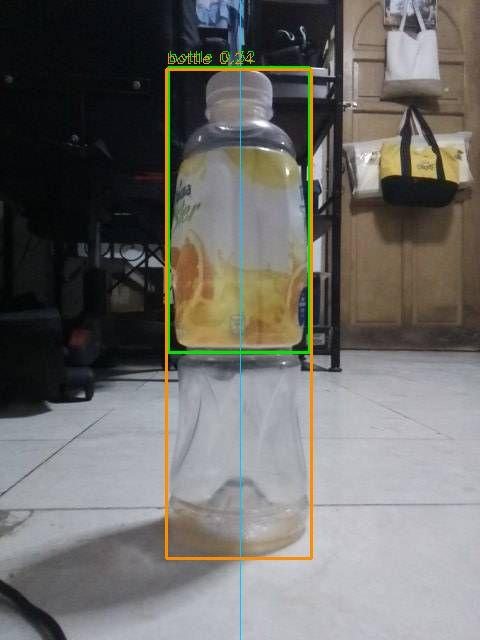
\includegraphics[width=0.44\columnwidth]{fig/detect.jpg}
\hfill
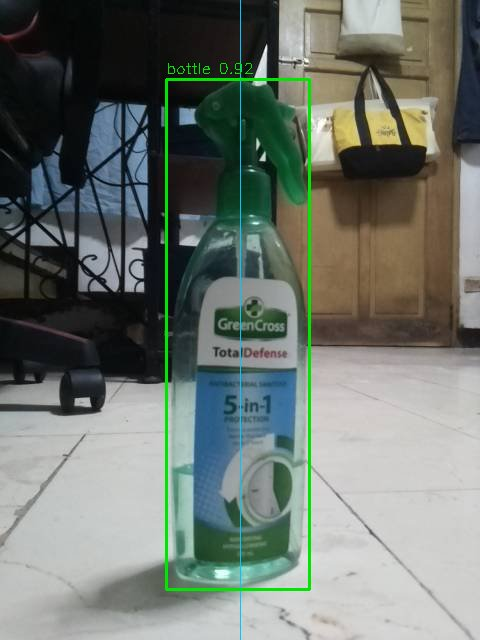
\includegraphics[width=0.44\columnwidth]{fig/arrived.jpg}
\caption{Left: detector output with the aim line the behaviour centres on.
Right: the robot at rest after a completed approach, $0.325$\,m from the target
against a $0.35$\,m goal.}
\label{fig:frames}
\end{figure}

Detection runs at approximately $19$\,ms per frame on a laptop RTX~3060, well
inside the camera's $5$\,Hz frame interval; perception is not the bottleneck.

Completed approaches to a floor-standing bottle stopped at $0.335$, $0.348$ and
$0.349$\,m against a $0.35$\,m goal, with bearing error remaining within
$\pm0.013$ (normalised image coordinates) throughout the approach phase. Range
decreased monotonically in each successful run.

\subsection{What these numbers do not show}

We state the limits plainly, as this is a work-in-progress report.
The successful trials number three, in a single room, with a single target
class, on one robot. There is no comparison against a calibrated
projection-based baseline, which is the natural control condition for our
central claim. Failure cases are catalogued diagnostically rather than
counted, so we cannot report a success rate. The stopping distances above are
drawn from runs that completed; runs aborted by the defects of
Sec.~\ref{sec:findings} are excluded, which biases the figure. A defensible
evaluation requires trials across several object classes, distances, lighting
conditions and clutter levels, with all attempts counted --- that is our
immediate next step, not a claim of this paper.

\section{Limitations}

The LiDAR observes only its own scan plane, roughly $18$\,cm above the floor.
Objects above it --- an item on a table --- are detected visually but cannot be
ranged, and the behaviour refuses to drive rather than estimate. Its $3.5$\,m
maximum range bounds the usable approach distance. The behaviour performs no
obstacle avoidance: it drives a straight line and stops for whatever is nearest
ahead, which may not be the target. Approaches cannot yet be composed with other
commanded motions. Finally, all tuning reported here is specific to this
platform, this room and this wireless link; the values are offered as evidence
of a method for obtaining them, not as constants.

\section{Conclusion}

We presented a language-directed object-approach behaviour that obtains bearing
from open-vocabulary vision and range from a planar LiDAR, deliberately
consuming them at different moments so that neither camera intrinsics nor
camera--LiDAR extrinsics are required. The behaviour works, stopping within
$1.5$\,cm of its goal in preliminary trials.

The more transferable result is the failure record. On this platform the
integration failures were overwhelmingly about sensor \emph{timing} --- a
transport delay created by publishing faster than the link could carry, a filter
with no path back from a bad reference, timers that ran while the robot was
deliberately not measuring, and a control gain that was safe only under the
assumption of a fresh image. Each presented as a perception failure and none
would have appeared in simulation. We suggest that reports of this kind, from
inexpensive and bandwidth-limited platforms, are a useful complement to
component-level benchmarks.

\section*{Acknowledgment}

Preliminary experiments were conducted in a domestic environment; we thank the
resident cat, whose unscheduled traversal of the robot's path exposed the
latching-filter defect of Sec.~\ref{sec:findings}.

\begin{thebibliography}{00}

\bibitem{saycan} M.~Ahn \emph{et al.}, ``Do as I can, not as I say: Grounding
language in robotic affordances,'' in \emph{Proc. Conf. Robot Learning (CoRL)},
2022.

\bibitem{codeaspolicies} J.~Liang \emph{et al.}, ``Code as policies: Language
model programs for embodied control,'' in \emph{Proc. IEEE Int. Conf. Robotics
and Automation (ICRA)}, 2023.

\bibitem{clip} A.~Radford \emph{et al.}, ``Learning transferable visual models
from natural language supervision,'' in \emph{Proc. Int. Conf. Machine Learning
(ICML)}, 2021.

\bibitem{owlvit} M.~Minderer \emph{et al.}, ``Simple open-vocabulary object
detection with vision transformers,'' in \emph{Proc. European Conf. Computer
Vision (ECCV)}, 2022.

\bibitem{groundingdino} S.~Liu \emph{et al.}, ``Grounding DINO: Marrying DINO
with grounded pre-training for open-set object detection,'' in \emph{Proc.
European Conf. Computer Vision (ECCV)}, 2024.

\bibitem{yoloworld} T.~Cheng \emph{et al.}, ``YOLO-World: Real-time
open-vocabulary object detection,'' in \emph{Proc. IEEE/CVF Conf. Computer
Vision and Pattern Recognition (CVPR)}, 2024.

\bibitem{ros2} S.~Macenski, T.~Foote, B.~Gerkey, C.~Lalancette, and W.~Woodall,
``Robot Operating System 2: Design, architecture, and uses in the wild,''
\emph{Science Robotics}, vol.~7, no.~66, 2022.

\end{thebibliography}

\end{document}
